\section*{Question 5}
\subsection*{a)}
The process has 15370 cases and 561470 events. Median number of events is 5 (and
average number The average duration is 48.8 weeks.

\subsection*{b)}

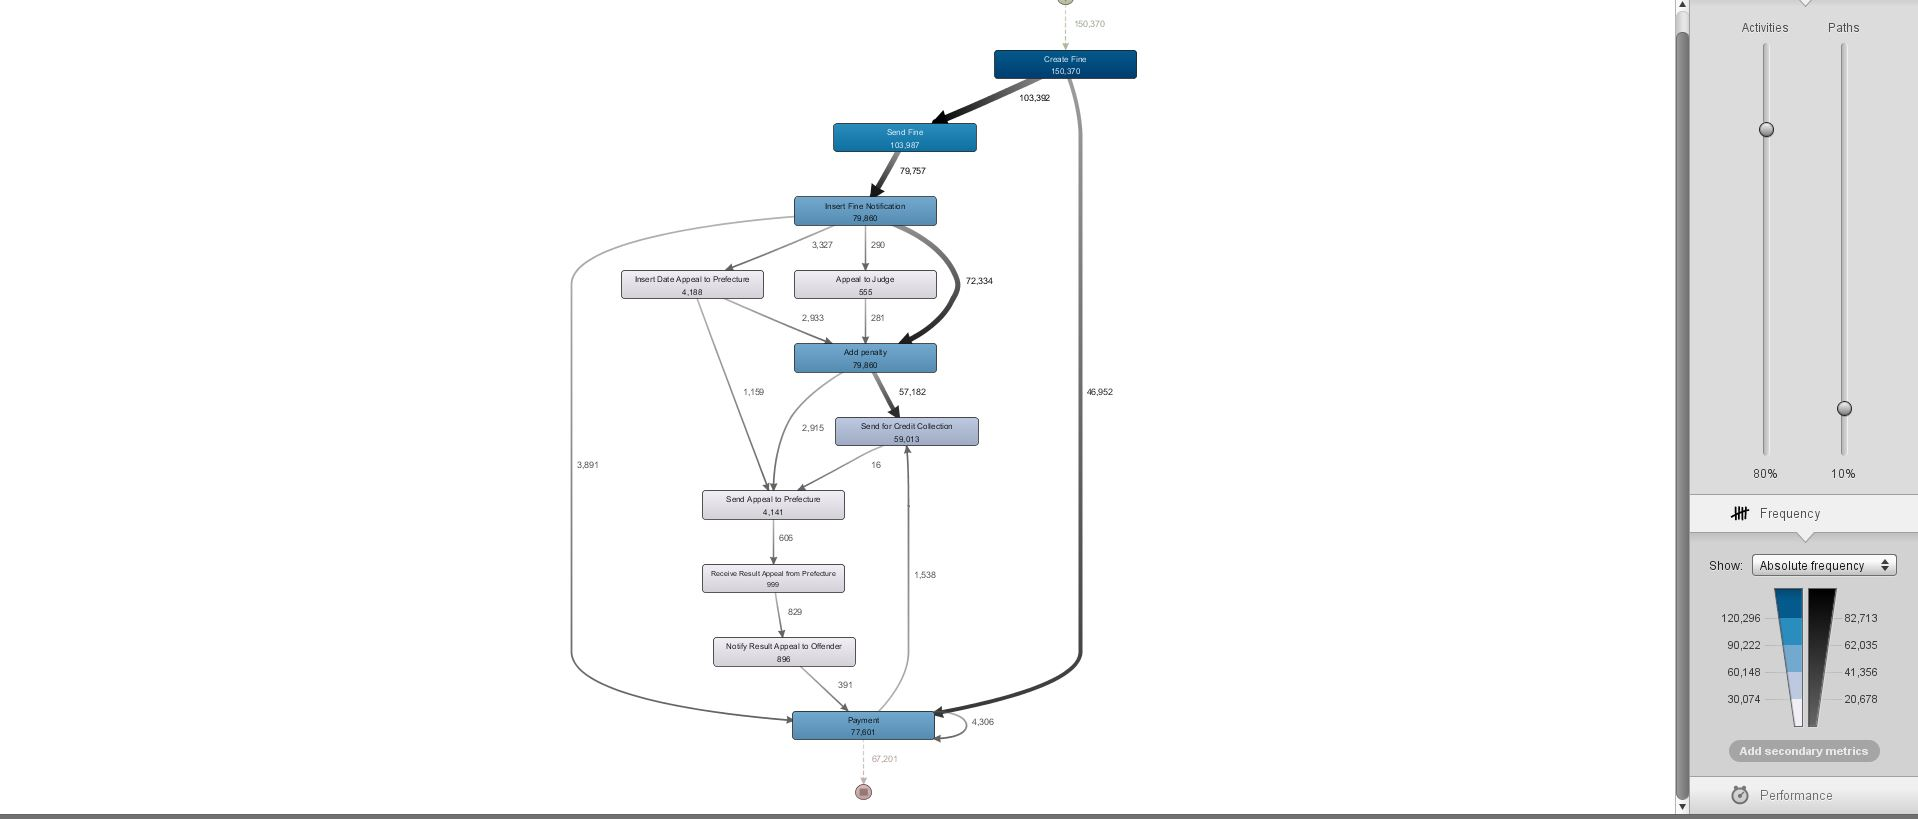
\includegraphics[width=0.8\textwidth]{Question5b.jpg}

The loop tells us, that a part of all people had to pay at least two times. If
you check the log data, you can see, that mostly it happens in the next 30 days.

It happen 4306 and for 4014 cases. So there are cases, where it happens more
than one time. You also can see, that it happens at most 14 times.

\subsection*{c)}
%Using Disco, analyze the time distribution of events over the time covered by this
%log? What is your interpretation of the distribution of events over the time?
% Do you see any remarkable patterns in the distribution of events (drifts, repeating
%behavior, etc.)?
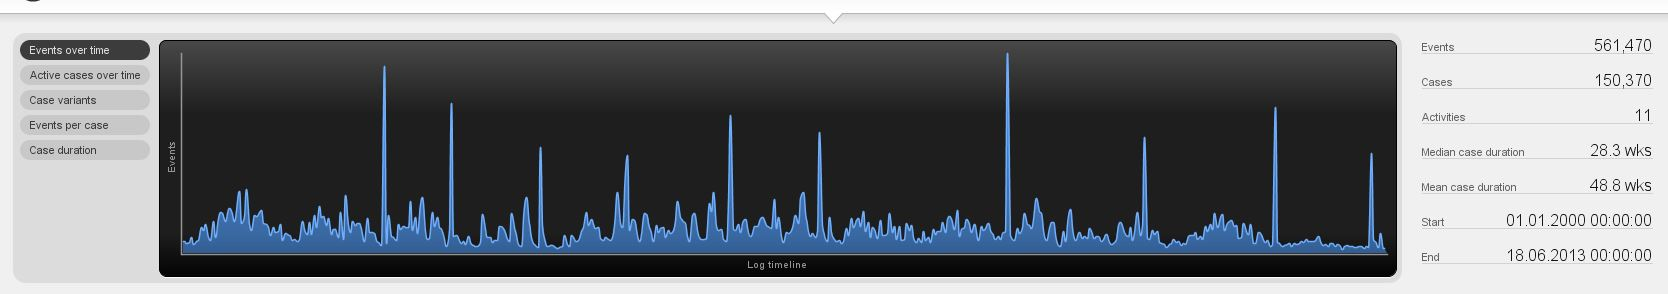
\includegraphics[width=0.8\textwidth]{Question5cDist.jpg}

You can see that the distribution is going up and down a little bit, but there
are 10 laces to see where more happens. Further in the end activity gets lower
and the distance between the 6th and 7th lace is higher than between the others.
It is always around the typical paydays, so probably a lot of people then have
the money to pay the fine.

\subsection*{d)}
% How many variants are in this event log? What is the size (number of process
% instances) of the third most frequent variant? Also, explain what happens in this
% variant (report the sequence of activities).
There are 231 variants. The third most frequent variant has 20385 instances. It
just contains the behaviour create and send fine. Nothing more happens there.

\subsection*{e)}
% Filter the event log using Disco while keeping 50% of the most common variants of
% process instances that finished until 01.01.2012 12: 12. What happens to the
% median and the average of case duration compared to the whole event log. Please
% also explain the difference between the median and the average (mean) of case
% duration.
It is just possible to $43\%$ or $56\%$. The average case duration shorts to
45.2 weeks and the median to 20.9weeks in both cases. So in average the cases
are faster finished.

The median is the instance in the middel. So if you write down all instances
sorted, it is the one in the middel. The average is the sum of all instances
divided by the number of instances. The average can change a lot for big or
extree small oultiers. The median shows more a real duration in the middle of
all instance durations.

\subsection*{f)}
% Discover the dotted chart view of the event log and interpret it using ProM. Adjust
% the Dotted chart settings in a way to answer question c. Are there any interesting
% (or odd) patterns in the dotted chart view that could explain the patterns found
% when answering question c?
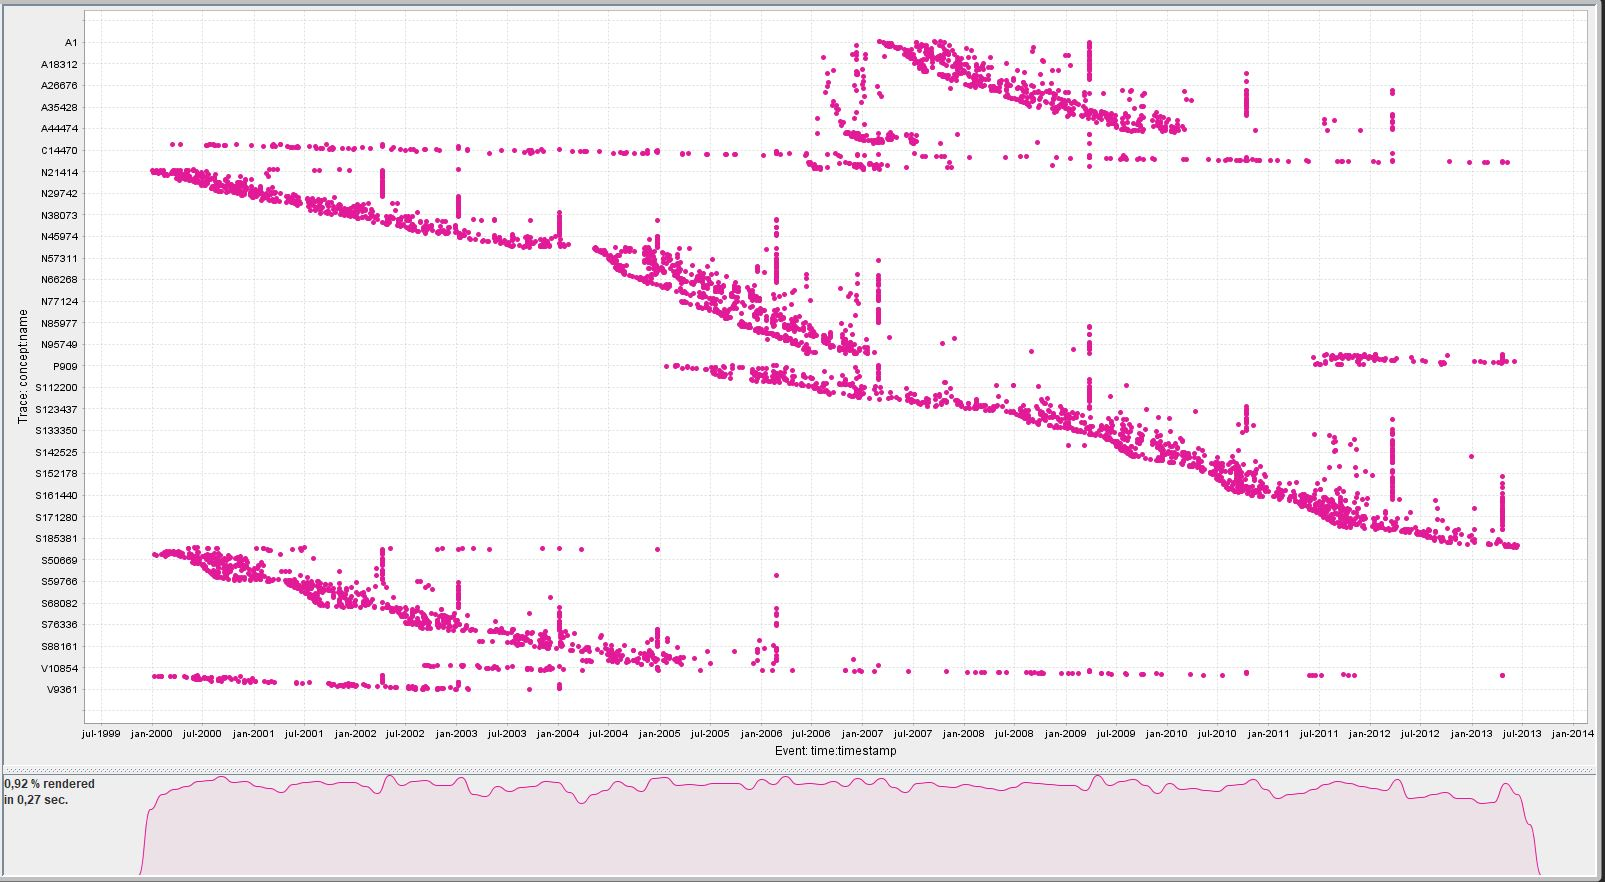
\includegraphics[width=0.8\textwidth]{Question5f.jpg}

In the first dotted chart you see when which case is active.

\includegraphics[width=0.8\textwidth]{Question5fc.jpg}

For interpreting the dot chart for the question c) I changed the y-axis to the
event names so I can see when which events happening. I also zoomed in so I can
see the months of the years. Now you can check better the dates of the peaks.

You can see that insert fine notification is strongly connected to the lashes to
see in c). Also a little bit the send fine.

Payment happens close to always but still is a little bit bundled at the peaks.

Furthermore I would say, that in disco it is more easy to see when peaks happen,
but in prom better to see what is happen on the peak days.

\subsection*{g)}
% Filter the event log using �filter log using simple heuristics� and then apply the
% Alpha algorithm (Alpha ++) on it. Filter the log appropriately. Show some insights
% that can only be seen after filtering.

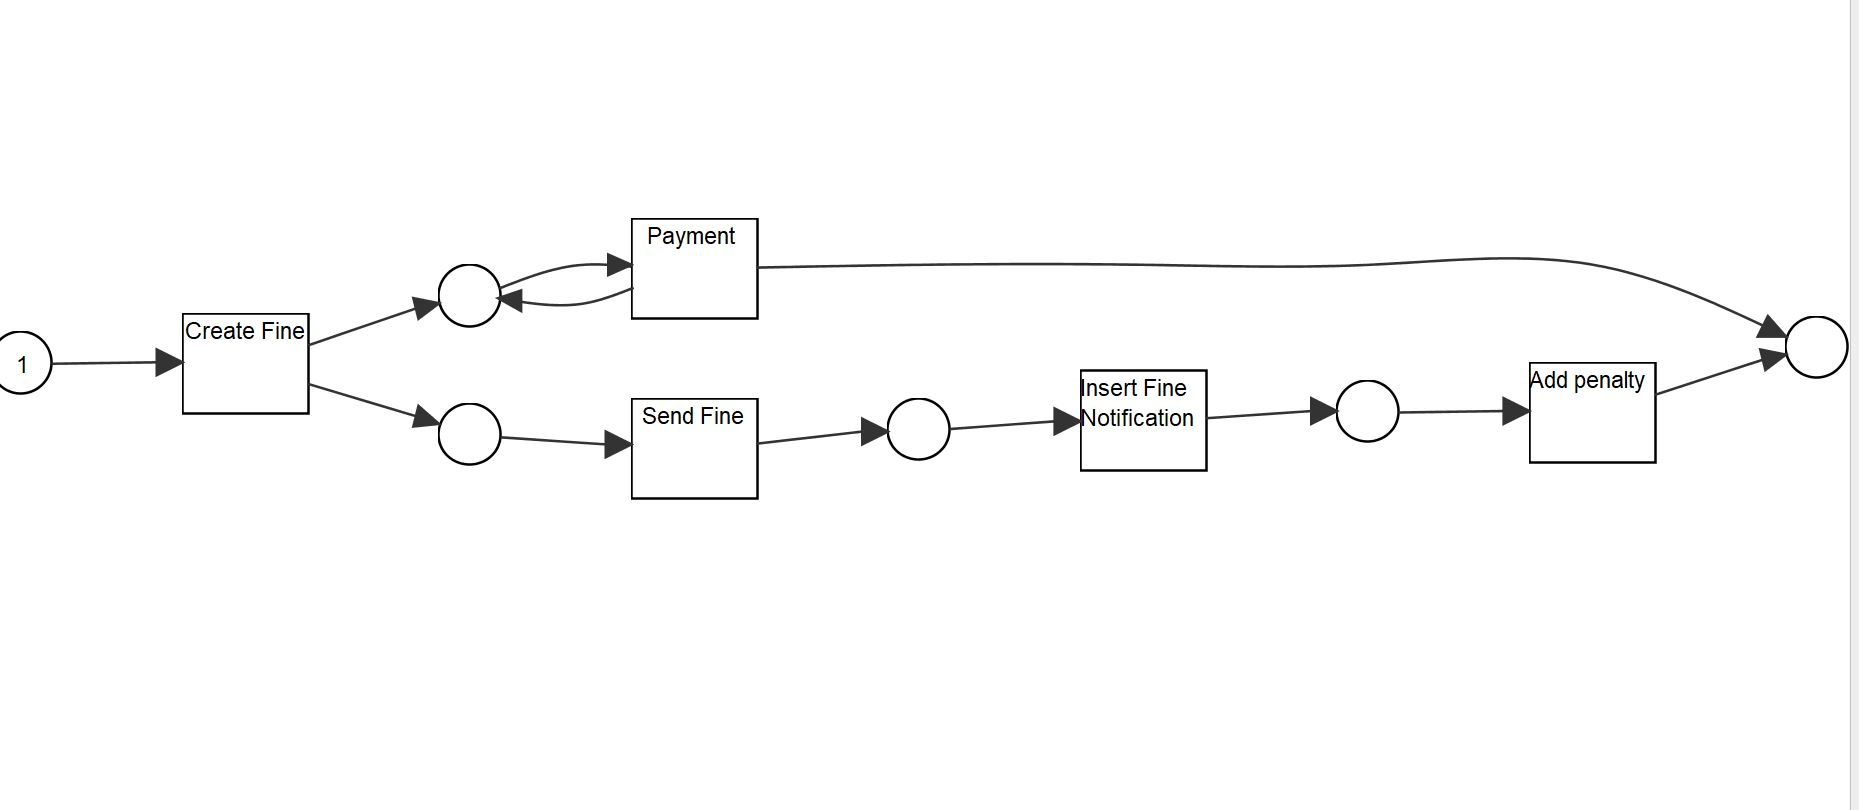
\includegraphics[width=\textwidth]{Question5g.jpg}

If you apply the alpha-algoirthm on the not filtered data you can not see so
clear, that in the resulting chart the payment can happen always and also
infinite often. It sounds weird, because you do not expect someone paying before
he gets the fine, but looking at the data it happens.

Also in the filtered version the people or pay after the fine is created or pay
to late, so that they get a penalty.

\subsection*{h)}
% Use the filtered event log in the previous question and this time use it as input for
% Disco. Which parts of the process are time consuming for most of the process
% instances? Answer this by interpreting the Disco model.

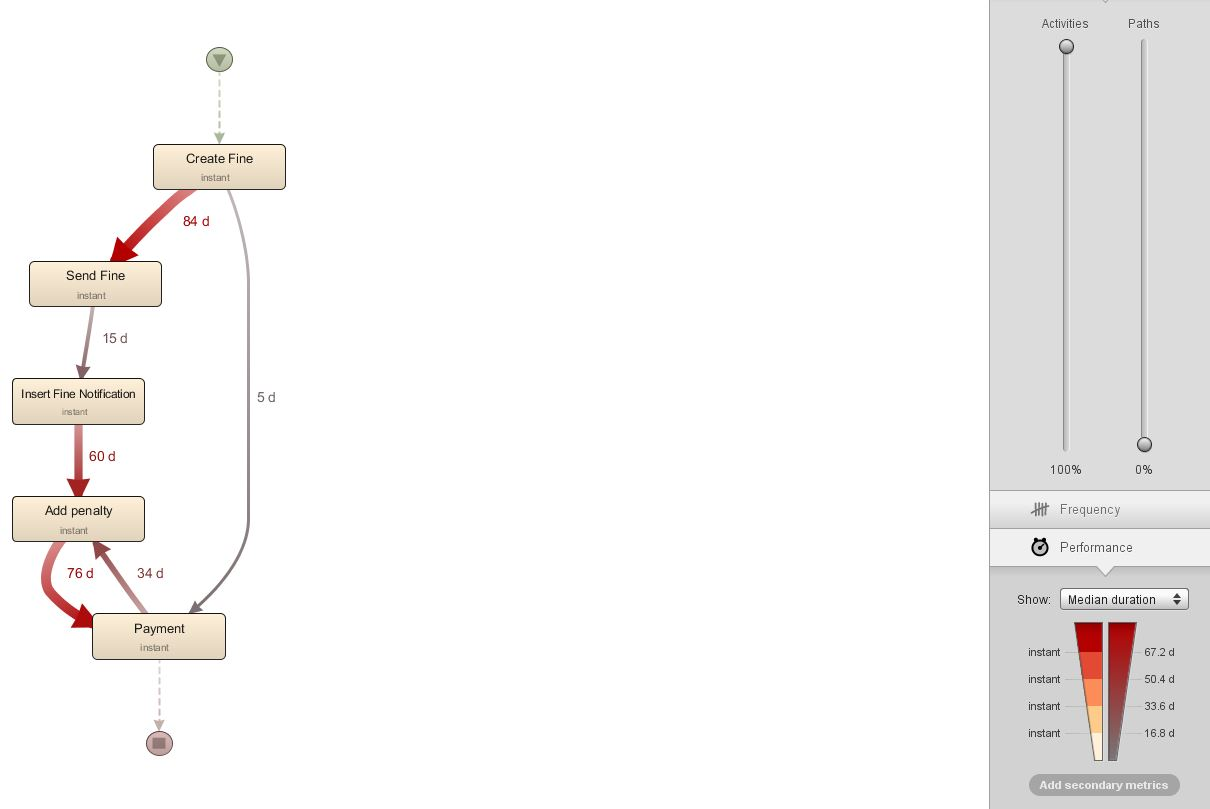
\includegraphics[width=\textwidth]{Question5h.jpg}

84days is the median for send fine. I chose the median, because then you get a
better idea what happens most of the times. The mean is 85.1 days.

What you also can see, is that after 60days always a penalty is added.
